\chapter{Architecture}
\section{Server}

\begin{figure}[hb]
\centering
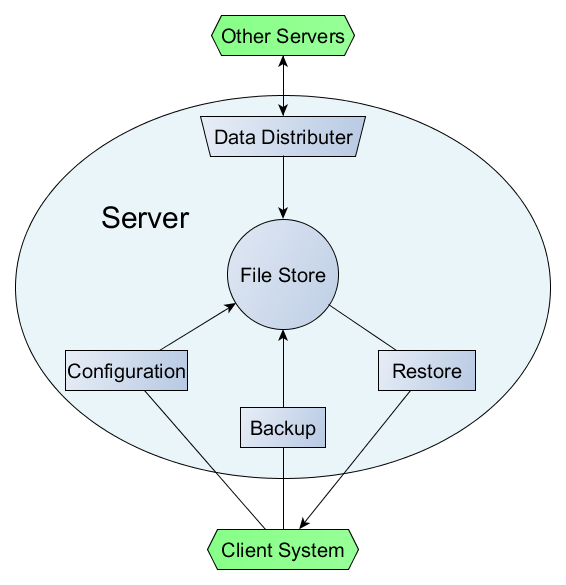
\includegraphics[scale=0.5]{images/architechure-diagram2.png}
\caption{A View of the Data Flow Through our Server}
\end{figure}

Our architecture is dual-layer. Each computer connects to a single storage
device and performs all backup operations to the device. Each computer will start
an OpenSSH server on boot. This, with the appropriate firewall settings, will
allow the storage device to contact the computer and access its files. The
storage device is made aware of the clients through a packet broadcast by the
client during setup. Once that initiation is complete the backup server can
connect to each client and download each file, block-wise. Each block is stored
in a database alongside its hash.
Documents associating files with a set of hashes and grouping files with
directories are stored in separate documents. Each computer is represented by a
document that specifies the files in that computer that are backed up in
addition to that computer's scheduling configuration. Once the data and its form
has been successfully stored, the data distributer is responsible for
finding other storage devices and replicating the data to each device.

%\section{Client}
%\begin{figure}[hb]
%\centering
%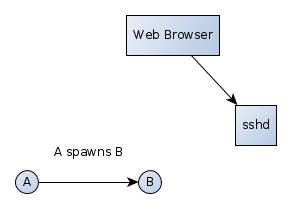
\includegraphics[scale=0.5]{images/client-arcitechure.png}
%\caption{A View of Client Architecture}
%\end{figure}
%
%The client's job is to find the server and provide a way for the server to connect with the client.

\section{Distribution Algorithm}

In order to distribute the backup data across our network, our system uses a
peer-to-peer networking algorithm based on Content Addressable Networks. \cite{scalable}
The algorithm is centered around the concept of a hash table that is shared by all the backup
servers in the network. The hash table is modeled as a square, and the backed up files are then
points that are hashed into this square. Each backup server in the network owns a rectangular portion
of this square, and is responsible for storing all the files whose points map into this rectangle.
This concept is shown in Figure \ref{fig:dht_1}. In this figure, in order to retrieve file 8 from the server,
it has to be retrieved from backup server 2.

\begin{figure}[hb]
\centering
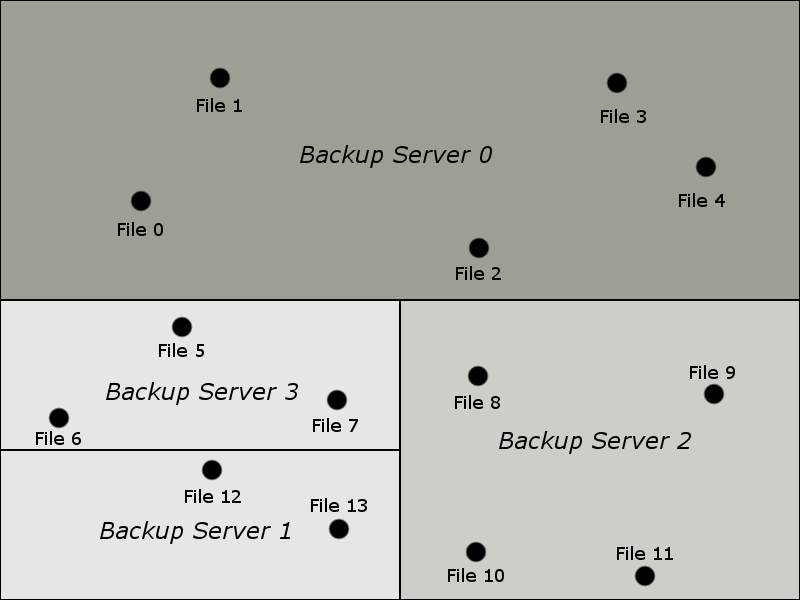
\includegraphics[scale=0.5]{images/dht_basic.png}
\caption{Distributed Hash Table}
\label{fig:dht_1}
\end{figure}

This algorithm has to take into account the fact that the network is chaotic and unstable.
Any backup server within the network can disappear from the network at any time and without warning.
Any backup server can also rejoin the network at any time. This is accounted for by the algorithm by
the way the network is structured. Each backup server in the network only communicates directly with
other servers that own a portion of the hash table adjacent to its own portion, called its neighbors.
For example, in Figure \ref{fig:dht_2}, backup server 2's neighbors are servers 4, 9, 3, and 8.

\begin{figure}[hb]
\centering
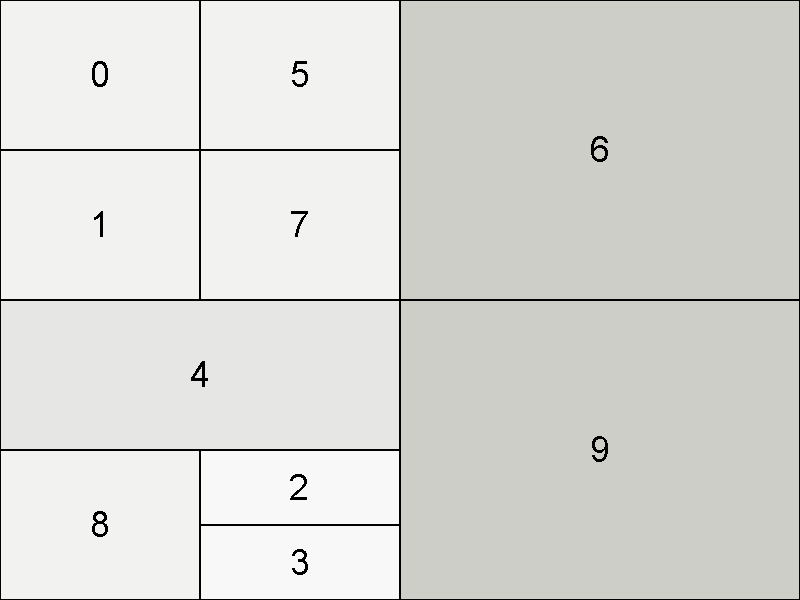
\includegraphics[scale=0.5]{images/dht_10_nodes.png}
\caption{Distributed Hash Table with 10 nodes}
\label{fig:dht_2}
\end{figure}

Then in order to deal with the fact that a backup server could disappear from the network at any time,
the neighbors of a backup server that goes down are responsible for taking over the space it occupied
in the hash table. Each backup server maintains consistent communication with its neighbors. If a server
is no longer responding to its neighbors, then those neighbors will negotiate to see who takes ownership
of the space the unresponsive server occupied in the hash table. In this way, each backup server is responsible
for maintaining the stability of the network near it in the hash table.
